% !TEX root = ../thesis-example.tex
%
%************************************************
% Grundlagen
%************************************************
\chapter{Grundlagen}
\label{sec:Grundlagen}

In diesem Kapitel werden wir die fachlichen Grundlagen zu unserem in Kapitel \ref{sec:Einfuehrung:Methodik} vorgestellten Lösungsansatz aufarbeiten. Dabei werden wir den Stand der Technik erklären, auf dem wir aufsetzen und diskutieren wie weit wir diesen nutzen können und wo wir diesen erweitern müssen. Wichtig hierfür ist das Verständnis, für die Problemstellungen in der Interaktion zwischen den Nutzern der Suche und der Suche selbst. Wir werden mögliche Lösungsansätze anschauen und darüber diskutieren. Um mit CTRs die Userrelevanz von Suchergebnissen bestimmen zu können, müssen wir lernen, Click-Through-Daten als Relevanz-Feedback zu deuten. Wie wir anschließend mithilfe dieses Relevanz-Feedbacks ein Reranking des Suchresultats durchführen, lernen wir in den Grundlagen zu unserem Reranking-Algorithmus. Diese Grundlagen sind notwendig für die Umsetzung des Lösungsansatzes in den nachfolgenden Kapiteln \ref{sec:Reranking} und \ref{sec:Implementierung}. 

% Grundbegriffe
%************************************************

\section{Grundbegriffe}
\label{sec:Grundlagen:Grundbegriffe}

In Kapitel \ref{sec:Grundlagen} und dem darauf folgenden Kapitel \ref{sec:Reranking}, werden Formeln mit selbst definierten Symbolen eingeführt. Folgend eine Legende der wichtigsten Symbole:

\begin{table}[H]
\centering
\vspace{-.5em}
\caption[Legende der wichtigsten Formel-Symbolen für den Algorithmus]{Legende der wichtigsten Formel-Symbolen für den Algorithmus}
\label{tab:LegendeSymboleFormelnAlgorithmus}
\vspace{-.5em}
\footnotesize
\renewcommand*{\arraystretch}{1.2}
\begin{tabular}{clcl} \hline
\textbf{Symbol} & \textbf{Bedeutung} & \textbf{Symbol} & \textbf{Bedeutung} \\ \hline
$u$	& ein Dokument im Suchergebnis & $C$	& das Dokument wird vom User \\ &&& im Suchergebnis angeklickt \\ 
$q$	& ein Suchterm & $E_{r_{u}}$	& ein Dokument wird aufgrund seiner Position $r$ \\ &&& im Suchergebnis angeschaut \\
$r$	& die Position des Dokumentes im Suchergebnis &  $A_{u}$	& das Dokument wird aufgrund seines Suchsnippets \\ &&& im Suchergebnis, zum Suchterm $q$ angeschaut \\ 
$c$	& ein Klick auf ein Dokument im Suchergebnis & $X_{u}$	& ein Zufallswert, der einem Dokument \\ &&& des Suchergebnisses zugewiesen wird \\
$s$ 	& der Suchvorgang zu einer Suchanfrage & $r_{X_{u}}$	& $r$ in der nach Zufallswert \\ &&& sortierten Liste der Suchergebnisse \\ 
$S$	& eine Sammlung von Suchvorgängen $s$ & $r_{P(C_{u})}$ 	& $r$ in der nach Klick-Wahrscheinlichkeit \\ &&& sortierten Liste der Suchergebnisse zum Suchterm $q$\\
$P$	& die Wahrscheinlichkeit dass ein Fall eintritt &  $R_{u}$	& durch den Reranking-Algorithmus berechneter \\ &&& Relevanz-Wert des Dokumentes $u$ \\
\hline
\end{tabular}
\vspace{-2em}
\end{table}

% Semantik von User-Interaktionen
%------------------------------------------------

\subsection{Semantik von User-Interaktionen}
\label{sec:Grundlagen:Grundbegriffe:SemantikUserInteraktionen}

\subsubsection{Problemstellungen der Click-Through-Daten: Was analysieren wir?}
\label{sec:Grundlagen:Grundbegriffe:SemantikUserInteraktionen:ProblemstellungenClick-Through-Daten}

\paragraph{Einzelne Wörter oder Teile des Suchterms können in weiteren Suchanfragen vorkommen}
Ein Suchterm kann aus einem oder mehreren Wörtern bestehen. Jeder User formuliert eine Suchanfrage anders. Sei es die Wortwahl, die Zeitform oder die Verwendung von Bindewörtern. Daraus lässt sich vermuten, dass einzelne Wörter oder Teile des Suchterms in weiteren Suchanfragen vorkommen können. Folglich muss der Suchterm semantisch aufgeschlüsselt werden, um Relationen zwischen den Click-Through-Daten und der Suchanfrage herstellen zu können. Nur so können wir alle relevanten Click-Through-Daten filtern.

\pagebreak

\paragraph{Suchanfragen mit Synonymen und verwandten Begriffen beachten}
Nehmen wir als Beispiel die Suchanfrage \glqq chronische Dyspnoe\grqq{}. Würden wir stattdessen den sinnverwandten Suchterm \glqq konstante Atemnot\grqq{} verwenden, würden wir für beide Fälle ähnliche Suchresultate erwarten. Folglich würden wir auch ähnliche Click-Through-Daten vermuten. Wir sollten daher die Synonyme und verwandten Begriffe zu unserem Suchterm ebenfalls beachten und deren Click-Through-Daten, in den Reranking-Algorithmus einfließen lassen. Dazu benötigen wir eine Wissensbasis, welche die Synonyme und verwandte Begriffe zu unserem Suchterm gespeichert hat. Eine solche Basis bieten Wörterbücher und Thesauri\footnote{Thesauri sind strukturierte Verzeichnisse von Begriffen, die allesamt in irgendeiner Beziehung zueinander stehen bezeichnet}. Beim Content von Springermedizin handelt es sich um \textit{medizinische Inhalte} in \textit{deutscher Sprache}. Es ergibt daher Sinn, dies in der Wahl der richtigen Wissensbasis zu berücksichtigen.

\subsubsection{Problemstellungen des Lösungsansatzes: Warum kann es schief gehen?}
\label{sec:Grundlagen:Grundbegriffe:SemantikUserInteraktionen:ProblemstellungenLoesungsansatz} 

Die folgenden Faktoren leiten sich aus dem verfolgten Lösungsansatz des Reranking-Algorithmus ab bzw. werden in diesem nicht beachtet. Wir müssen davon ausgehen, dass diese das Untersuchungsergebnis des Lösungsansatzes negativ beeinflussen könnten.

\paragraph{Die Relation des Suchterms zu den Click-Through-Daten wird nicht gewichtet}
Die Click-Through-Daten sind dann relevant, wenn mindestens ein Wort des aufgeschlüsselten Suchterms, in Relation zu diesen Daten steht. Dadurch können falsche Relationen entstehen und nicht relevante Click-Through-Daten, die Klick-Wahrscheinlichkeiten der Dokumente im Reranking-Algorithmus negativ beeinflussen.

\paragraph{Intentionen und die Mehrdeutigkeit von Suchbegriffen werden nicht beachtet}
Die genaue semantische Analyse eines Suchterms beinhaltet unter anderem die Erkennung von Begriffen und deren Mehrdeutigkeiten. Suchte jemand z.B. nach dem Begriff \glqq Brücke\grqq{}, hat dieser im medizinischen Kontext mehrere Bedeutungen. Es könnte \glqq ein Teil des zentralen Nervensystems\grqq{} gemeint sein oder \glqq eine Form des Zahnersatzes\grqq{}. Wie bereits im vorherigen Kapitel \ref{sec:Grundlagen:Grundbegriffe:SemantikUserInteraktionen:ProblemstellungenClick-Through-Daten} erwähnt, können wir mithilfe eines Thesaurus, die verschiedenen Bedeutungen erkennen. Der Thesaurus könnte uns zu dem Begriff \glqq Brücke\grqq{} beispielsweise, folgende Informationen zurückgeben:

\begin{figure}[H]
\centering
\begin{minipage}{0.45\linewidth}
        \centering
        \vspace{-2em}
		\caption[Im Thesaurus gespeicherte Werte zum Suchterm \glqq Brücke\grqq{}]{Im Thesaurus gespeicherte Werte zum Suchterm \glqq Brücke\grqq{}}
		\label{fig:ThesaurusBruecke}
		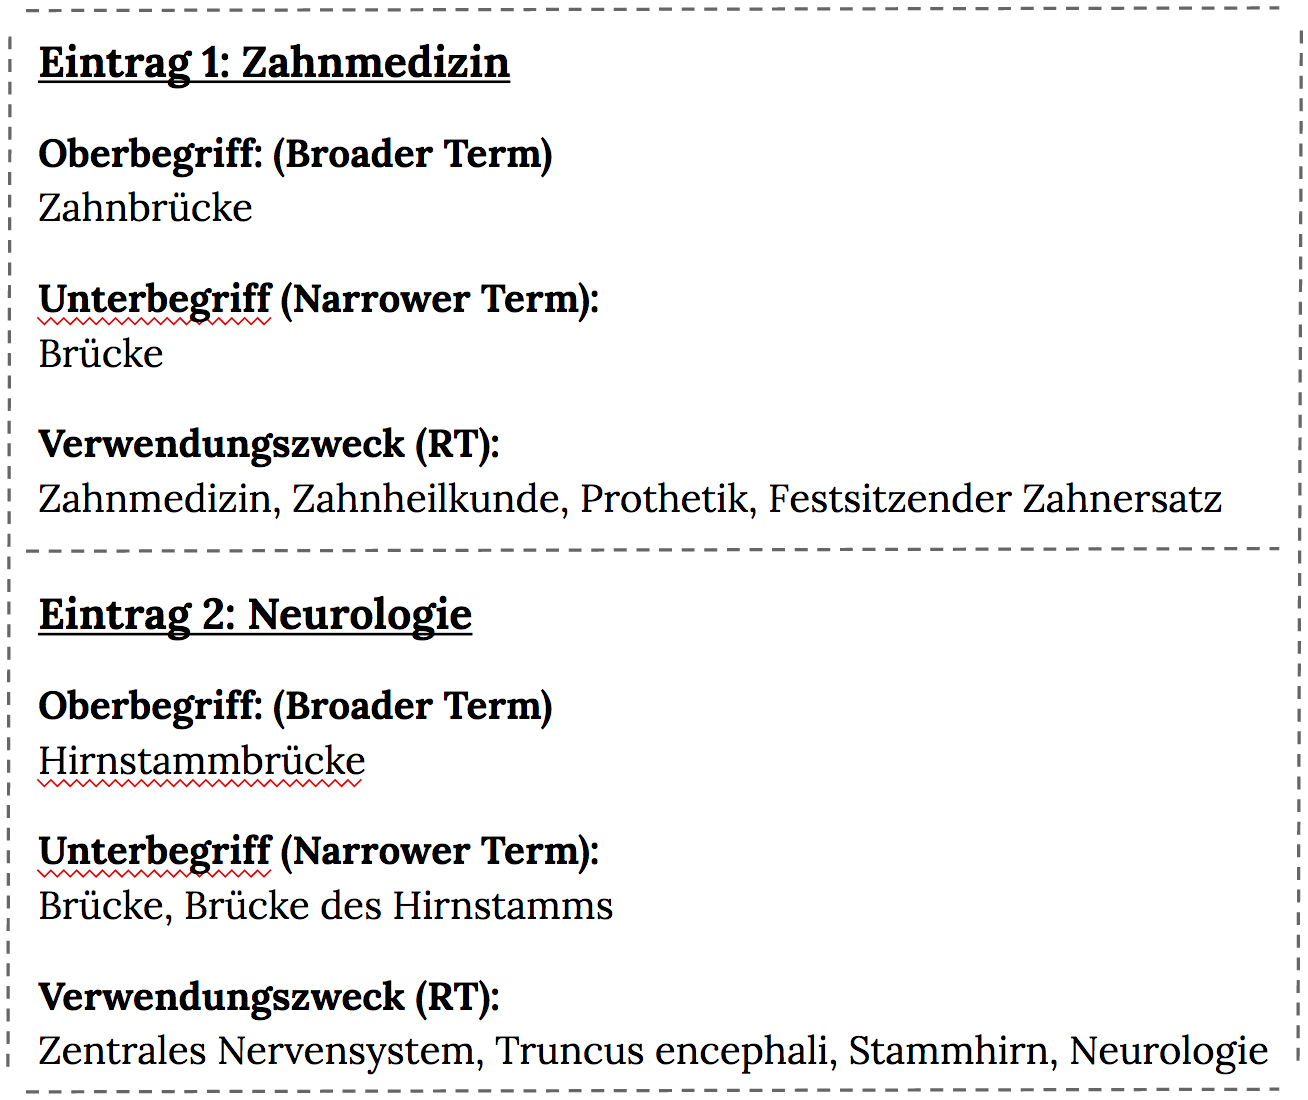
\includegraphics[width=\linewidth]{gfx/BeispielMehrdeutigkeit}
		\vspace{-3em}
    \end{minipage}
    \hfill
    \begin{minipage}{0.45\linewidth}
        Unser Reranking-Algorithmus ignoriert diese Mehrdeutigkeit. Er würde in diesem Fall alle Click-Through-Daten zu beiden Begriffsbedeutungen suchen. Hier können wir zufallsbedingt drei Ausgangslagen haben. Die Click-Through-Daten entsprechen der Suchintention (1) - das wäre der zufallsbedingte Optimalfall. Das Suchresultat wird von der Mehrfachbedeutung nicht beeinflusst. Das Gegenteil tritt ein (2) - das Suchresultat wird in diesem Fall durch eine falsche Relevanz negativ beeinflusst. Es sind keine Click-Through-Daten vorhanden (3) - die Solr und die Klick-Wahrscheinlichkeit der Position im Suchresultat, definieren das Suchergebnis. In diesem Fall kann die Wertigkeit des Algorithmus nicht vorhergesehen werden.
    \end{minipage}
\end{figure}

\paragraph{Keine Aktualität in der Suche}
Der von uns verfolgte Reranking-Algorithmus nimmt keine Rücksicht auf die \glqq Aktualität\grqq{} eines Beitrages sondern nur auf die Klick-Wahrscheinlichkeit und kann dadurch, aktuellere Dokumente trotz Relevanz, schlecht positionieren im Suchresultat.  Die Klick-Wahrscheinlichkeit kann durch zwei Faktoren beeinflusst werden. Hohe Relevanz in der Solr-Suche (1) - wird in der Volltextsuche die Aktualität des Dokumentes in die Berechnung der Relevanz einbezogen, werden aktuelle Beiträge im Suchergebnis der Solr weit vorne eingestuft. Wie wir aus Abb. \ref{fig:Grundlage:AnalyseKlicksPositionen} erkennen können, haben die ersten Positionen des Suchergebnisses eine höhere Klick-Wahrscheinlichkeit. Das könnte die Berechnung des Reranking-Algorithmus positiv beeinflussen. Reranking-Algorithmus um Zufallsfaktor erweitern (2) - mithilfe eines Zufallsfaktor ist die Reihenfolge der Suchresultate weniger vom Algorithmus abhängig und die Wahrscheinlichkeit, aktuelle Dokumente ohne Click-Through-Daten weit vorne im Suchergebnis zu finden, wird erhöht.

\paragraph{Interessante Dokumente werden nie gesehen}
Wie bereits oben erwähnt, beachtet der Reranking-Algorithmus Dokumente ohne Click-Through-Daten nur, wenn die Position im Suchresultat eine Klick-Wahrscheinlichkeit aufweist. Dadurch kann es sein, dass interessante Dokumente nie gesehen werden. Dem entgegenwirken können wir ebenfalls mit dem oben erwähnten Zufallsfaktor. Dadurch wird die Klick-Wahrscheinlichkeit für interessante Dokumente zufallsbedingt erhöht.

\subsubsection{Nicht beeinflussbare Faktoren: Fehlerhafter Content verfälscht die Suchergebnisse}
\label{sec:Grundlagen:Grundbegriffe:SemantikUserInteraktionen:FehlerhafterContent}

Die folgenden Faktoren beeinflussen das Suchergebnis negativ, sind aber vom Content so vorgegeben. Der von uns verfolgte Lösungsansatz des Reranking-Algorithmus kann diese nicht beeinflussen. Wir beachten diese Faktoren in unserer Arbeit darum nicht.

\paragraph{Mehrfachverwertung des Contents}
Auf der Springermedizin Suche wird teilweise im Suchergebnis auf denselben Artikel mehrfach  verwiesen. Das liegt an der bei Springermedizin praktizierten Mehrfachverwertung des Contents. Es gibt \textit{Journal-Artikel}, das sind aus Journalen, Zeitschriften oder Magazinen stammende Artikel, die auf Springermedizin direkt online\footnote{Der Begriff \glqq online\grqq{} wird hier als Verweis auf die Springermedizin.de-Webseite verwendet} gelesen werden können. Bei Neuerscheinung des Artikels, werden dazu oft \textit{redaktionelle Artikel} publiziert, welche auf den Journal-Artikel verweisen sollen. Diese können im CMS (siehe Abb. \ref{fig:SucheSpringerNature}) von der Suche exkludiert werden. Werden diese nicht exkludiert, können beide Artikel im Suchergebnis erscheinen.

\paragraph{Ausspielung von Teaser}
Springermedizin verwendet Teaser\footnote{Als Teaser wird ein kurzer Texte bezeichnet, der das Interesse für den nachfolgenden Beitrag wecken soll} auf der Startseite und auf Übersichtsseiten zu Rubriken, als Einstieg in den nachfolgenden, ausführlichen Beitrag. Diese werden auch in der Suche ausgespielt. Teaser sagen nichts über die Wertigkeit des Beitrages aus. Es wird nicht bekanntgegeben, auf welche Art von Beitrag (z.B. wissenschaftliche Publikation oder ein Artikel aus einem Journal) verwiesen wird und von welchem Autor der Beitrag stammt. Teaser können darum nicht nach Relevanz eingestuft werden und sollten nicht im Suchergebnis erscheinen.

\paragraph{Fehlerhafte Importe der Daten}
Viele Beiträge sind falschen Rubriken zugeordnet. Beispielsweise werden Beiträge fälschlicherweise als wissenschaftliche Publikationen publiziert, obwohl sie aus einem Journal oder einer Fachzeitschrift stammen. Diese Fehler sind auf fehlerhafte Importe der Daten zurückzuführen und verfälschen die Wertigkeit des Suchergebnisses.

\paragraph{Schlechte Suchsnippets beeinflussen die Klick-Wahrscheinlichkeit eines Dokumentes negativ}
Das PBM berechnet die Klick-Wahrscheinlichkeit, also die \textit{Attraktivität} eines Dokumentes auf Basis dessen Klick-Häufigkeit zum Suchterm und dessen Position im Suchresultat. Das heißt, der User analysiert das Suchresultat und sobald er auf den Link zu einem Dokument klickt, fließt dieser Klick in die Berechnung ein. Folglich bestimmt nicht der Inhalt des Dokumentes über dessen Attraktivität, sondern dessen Suchsnippet\footnote{Unter einem Suchsnippet wird eine Zusammenfassung des Inhalts des verlinkten Dokumentes als kurzen Teasertext verstanden}. Wirkt dieses wenig relevant, kann dadurch die Klick-Wahrscheinlichtkeit negativ beeinflusst werden.

\pagebreak

\subsubsection{Analyse der Click-Through-Daten: Wenige Dokumente erhalten viele Klicks}
\label{sec:Grundlagen:Grundbegriffe:SemantikUserInteraktionen:DocumentAttraction}


Um das Klick-Verhalten der User auf der Springermedizin-Suche zu verstehen, ist es wichtig anhand oft gesuchter Suchphrasen dieses Verhalten zu analysieren. Dazu wurde eine Analyse über einen Zeitraum von 30 Tagen erstellt und die zehn am häufigsten gesuchten Suchphrasen verwendet. Die Analyse vergleicht für jede Suchphrase die 20 Dokumente mit den meisten Klicks. Die Dokumente wurden hierbei nicht nach Position im Suchergebnis sondern nach Klick-Häufigkeit selektiert. Jeder Graph der folgenden Abbildung \ref{fig:Grundlagen:AnalyseKlicksTop10Suchergebnisse} stellt eine Suchphrase dar. Wie wir sehen, zeigen die meisten Graphen ein exponentiell stark abnehmendes Verhalten der Klick-Häufigkeiten. Dieses exponentielle Verhalten zeigt, dass einzelne Dokumente häufig und viele Dokumente selten bis nie angeklickt werden. Dieser Effekt kann wie in vielen natürlichen Phänomenen mit exponentiellem Verhalten, durch das Potenzgesetz (Power Law, siehe \cite{PowerLaw}) beschrieben werden. 

\begin{figure}[H]
\centering 
\vspace{-1em}
\caption[Analyse der 20 am häufigsten angeklickten Dokumente  der zehn meistgesuchten Suchphrasen. \textit{Zeitraum der Analyse: 19.08.16 - 19.09.16}]{Analyse der 20 am häufigsten angeklickten Dokumente  der zehn meistgesuchten Suchphrasen. \\ \textit{Zeitraum der Analyse: 19.08.16 - 19.09.16}}
\label{fig:Grundlagen:AnalyseKlicksTop10Suchergebnisse}
 
\pgfplotstableread[col sep=semicolon]{content/diagrams/clicks_top10_searchphrases_result.csv}\topSearchphrases
  
\begin{tikzpicture}
\begin{axis}[
	width=14cm,
	height=5cm,
	scale only axis,
	xmajorgrids,
	xminorgrids,
    ylabel=\textbf{Anzahl der Klicks}, 
	xlabel=\textbf{Dokumente sortiert nach Anzahl der Klicks},
    xtick=data,
    ymin=0,
    xmin=1,
    xmax=20,
    legend pos=north east,
    legend style={font=\tiny}
]
\addplot table [
    x=S1,
    x=Position
] {\topSearchphrases};
\addplot table [
    y=S2,
    x=Position
] {\topSearchphrases};
\addplot table [
     y=S3,
    x=Position
] {\topSearchphrases};
\addplot table [
     y=S4,
    x=Position
] {\topSearchphrases};
\addplot table [
     y=S5,
    x=Position
] {\topSearchphrases};
\addplot table [
     y=S6,
    x=Position
] {\topSearchphrases};
\addplot table [
     y=S7,
    x=Position
] {\topSearchphrases};
\addplot table [
     y=S8,
    x=Position
] {\topSearchphrases};
\addplot table [
     y=S9,
    x=Position
] {\topSearchphrases};
\addplot table [
     y=S10,
    x=Position
] {\topSearchphrases};
\legend{borreliose ($1015$ Suchergebnisse), copd ($17337$ Suchergebnisse), dgrm-jahrestagung $2016$ ($18$ Suchergebnisse), diabetes ($148755$ Suchergebnisse), dyspnoe ($10601$ Suchergebnisse), forensische traumatologie ($150$ Suchergebnisse), gicht ($1188$ Suchergebnisse), hypertonie ($12765$ Suchergebnisse), mmw ($12666$ Suchergebnisse), vorhofflimmern ($4981$ Suchergebnisse)}
\end{axis}
\end{tikzpicture}

\vspace{-2em}
\end{figure}

Betrachten wir die Graphen, können wir vor allem für die ersten fünf analysierten Dokumente verglichen mit den restlichen analysierten Dokumenten, hohe Klick-Häufigkeiten feststellen. Daraus lässt sich die Vermutung ableiten, dass einzelne Dokumente eine sehr hohe Relevanz für die entsprechende Suchanfrage aufweisen und nur wenige Dokumente auf die User als relevant wirken. Ein weitere Vermutung ist, dass der zu durchsuchende Content wenig relevante Dokumente hat. Die Suchphrasen lassen auf sehr diverse Suchintentionen deuten. Es handelt sich hierbei unter anderem um Krankheiten, Zeitschriften und Behandlungen mit mehreren tausend Suchergebnissen. Die Wahrscheinlichkeit, dass wenig relevanter Content für die meisten der analysierten Suchphrasen zutrifft, sollte aufgrund der hohen Anzahl an gefundenen Suchergebnissen zu diesen Suchphrasen, relativ gering sein. Wir müssen darum eher davon ausgehen, dass sich die User auf einzelne im Suchresultat weit oben stehende Dokumente festfahren. Das könnte an schlechten Suchergebnissen und somit an einer schlechten Suchqualität liegen. Um jedoch ein genaueres Bild über das Verhalten erstellen zu können müssen wir einen Vergleich mit der nachfolgenden Analyse in Abbildung \ref{fig:Grundlage:AnalyseKlicksPositionen} ziehen.

\subsubsection{Analyse der angeklickten Positionen: Die ersten Positionen werden häufiger angeklickt}
\label{sec:Grundlagen:Grundbegriffe:SemantikUserInteraktionen:RankExamination}


In der unten folgenden Analyse sehen wir das positionsbezogene Klick-Verhalten der User auf der Springermedizin-Suche. Dazu wurden über den Zeitraum von einem Monat, die letzten 1000 Suchanfragen ausgewertet. Dargestellt sehen wir die Häufigkeitsverteilung der Klicks als Graph. Wir beschränken uns hierbei auf die ersten 20 Positionen der Suchresultate. Wie wir sehen, nimmt die Anzahl der Klicks mit zunehmender Position exponentiell ab. Dieser Effekt kann ebenfalls, wie in Abb. \ref{fig:Grundlagen:AnalyseKlicksTop10Suchergebnisse}, durch das Potenzgesetz (Power Law, siehe \cite{PowerLaw}) beschrieben werden. 

\begin{figure}[H]
\centering 
\vspace{-1em}
\caption[Analyse der Klicks auf die ersten 20 Positionen der Suchergebnisse aller Suchanfragen. \textit{Zeitraum der Analyse: 19.08.16 - 19.09.16}]{Analyse der Klicks auf die ersten 20 Positionen der Suchergebnisse aller Suchanfragen. \\ \textit{Zeitraum der Analyse: 19.08.16 - 19.09.16}}
\label{fig:Grundlage:AnalyseKlicksPositionen}

\footnotesize
\pgfplotstableread[col sep=semicolon]{content/diagrams/clicks_top1000_ranks_result.csv}\topRanks
  
\begin{tikzpicture}
\begin{axis}[
	width=14cm,
	height=3cm,
	scale only axis,
	xmajorgrids,
	xminorgrids,
    ylabel=\textbf{Anzahl der Klicks}, 
	xlabel=\textbf{Position im Suchergebnis},
	nodes near coords, 
	 every node near coord/.append style={xshift=+10pt,yshift=-1pt},
    xtick=data,
    ymin=0,
    xmin=1,
    xmax=20,
    legend style={font=\tiny}
]
\addplot table [
    x=Position,
    y=Klicks
] {\topRanks};
\legend{Anzahl Klicks}
\end{axis}
\end{tikzpicture}

\vspace{-2em}
\end{figure}

Betrachten wir den Graphen, sehen wir, dass besonders die erste Position, auffällig oft angeklickt wird. Daraus könnten wir die Vermutungen ableiten, dass die Suche eine sehr gute Qualität besitzt, weil die zu oberst angezeigten Dokumente, sehr relevant sind und die meisten User der Suchmaschine vertrauen. Wie wir aus den Analysen von \cite{Joachims} lesen können, müssen wir davon ausgehen, dass die Häufigkeit des Klicks auf die ersten Positionen des Suchresultates eher dem Vertrauen der User der Suchmaschine, als der Qualität der Suche geschuldet ist. Vergleichen wir die Analyse aus Abb. \ref{fig:Grundlagen:AnalyseKlicksTop10Suchergebnisse} mit dieser Analyse, sehen wir ein sehr ähnliches Muster in der Häufigkeitsverteilung der Klicks. Wir können anhand der Klick-Zahlen ebenfalls vermuten, dass die am häufigsten angeklickten Dokumente, sich dabei auf den ersten Positionen des Suchergebnisses befunden haben.

% Userrelevanz mittels CTR
%------------------------------------------------

\subsection{Userrelevanz mittels CTR}
\label{sec:Grundlagen:Grundbegriffe:Click-Through-Daten}

Um mit Click-Through-Daten arbeiten zu können, müssen wir zuerst verstehen, was Click-Through-Daten sind und wie sie entstehen. 

\subsubsection{Was sind Click-Through-Daten und wie entstehen diese?}
\label{sec:Grundlagen:Grundbegriffe:Click-Through-Daten:WasSindClick-Through-Daten}

Click-Through-Daten sind Tracking-Daten. Tracking-Daten entstehen durch die Interaktion zwischen dem User der Applikation und der Applikation selbst. Sie verfolgen das Verhalten der User auf der Applikation und speichern dieses in einer Datenbank, in unserem Fall in Webtrekk ab. Die für uns interessanten Tracking-Daten entstehen, wenn der User auf der Suche von Springermedizin ein Anfrage stellt und darauf folgend, ein Element aus dem Suchresultat anklickt.

\subsubsection{Wie werden die Click-Through-Daten in Webtrekk gespeichert?}
\label{sec:Grundlagen:Grundbegriffe:Click-Through-Daten:SpeichernClick-Through-Daten}

Die Speicherung der Daten auf Webtrekk übernimmt die Springermedizin-Applikation. Führt ein User eine Suche durch und klickt dabei ein Resultat an, sendet die Springermedizin-Applikation die Tracking-Informationen an Webtrekk. Die Tracking-Daten für diese Aktion, setzen sich zusammen aus der Suchanfrage, dem Zeitpunkt der Suche, den Userdaten, der angeklickten Position im Suchresultat und den Dokumentinformationen zum angeklickten Dokument.

\subsubsection{Wie können wir Click-Through-Daten aus Webtrekk lesen?}
\label{sec:Grundlagen:Grundbegriffe:Click-Through-Daten:LesenClick-Through-Daten}

Webtrekk ist ein Analysetool. Das heißt für uns, wir können nicht direkt auf die Datenbank mit den Tracking-Daten zugreifen. Um die Tracking-Daten lesen zu können, müssen wir eine Analyse auf Webtrekk ausführen. Mithilfe dieser Analyse können wir uns die Click-Through-Daten so zusammenstellen lassen, wie wir sie für die Berechnung der CTR benötigen.

\paragraph{Klick-Häufigkeiten zu Suchterm selektieren und mittels Filtern einschränken} 
Die Click-Through-Daten bestehen aus einzelnen \textit{Klick-Häufigkeiten}. Eine Klick-Häufigkeit beschreibt die Anzahl der Klicks, die zu einer bestimmten Suchanfrage auf ein bestimmtes Dokument gemacht wurden und auf welcher Position im Suchresultat, sich dieses Dokument dabei befunden hat. Die Webtrekk-Analysen geben uns eine Sammlung von Klick-Häufigkeiten zurück. Wir können bei diesen Analysen die Klick-Häufigkeiten nach Suchbegriffen filtern und den Zeitraum mitgeben, in welchen die Suchanfragen durchgeführt wurden. Des weiteren gibt es die Möglichkeit, weitere Filter wie die Anzahl zurückzugebender Klick-Häufigkeiten oder auch den \glqq Login-Status\footnote{Mit Login-Status wird zwischen einem zum Zeitpunkt der Suche auf der Springermedizin-Applikation angemeldeten und nicht angemeldeten Usern unterschieden} des Users\grqq{} zu setzen. 

\subsubsection{Wie sehen die Click-Through-Daten aus?}
\label{sec:Grundlagen:Grundbegriffe:Click-Through-Daten:AussehenClick-Through-Daten}

Eine Beispiel einer Klick-Häufigkeit, wie sie von einer Webtrekk-Analyse ausgespielt wird, sieht wie folgt aus:

\begin{table}[H]
\centering
\vspace{-.75em}
\caption[Beispiel Click-Through-Daten]{Beispiel Click-Through-Daten}
\vspace{-.5em}
\label{tab:BeispielCTDaten}
\footnotesize
\renewcommand*{\arraystretch}{1.2}
\resizebox{\textwidth}{!}{%
\begin{tabular}{|lc|}\hline
	\textbf{Click-Through-Daten} & \textbf{Klick-Häufigkeit} \\ \hline
	searchresult-1.Course.chronische Dyspnoe bei Erwachsenen.10621768.chronische Dyspnoe & 5 \\ \hline
 \end{tabular}
 }
\vspace{-2em}
\end{table}

Hier die Aufschlüsselung der Click-Through-Daten:

\begin{table}[H]
\centering
\vspace{-.75em}
\caption[Beispielhafte Aufschlüsselung der Click-Through-Daten]{Beispielhafte Aufschlüsselung der Click-Through-Daten}
\label{tab:AufschluesselungCTDaten}
\vspace{-.5em}
\footnotesize
\renewcommand*{\arraystretch}{1.2}
\resizebox{\textwidth}{!}{%
\begin{tabular}{|lllll|}\hline
	\textbf{Position} & \textbf{Dokumenttyp} & \textbf{Titel} & \textbf{ID} & \textbf{Suchterm} \\ \hline
	searchresult-1 & Course & chronische Dyspnoe bei Erwachsenen & 10621768 & chronische Dyspnoe \\ \hline
\end{tabular}
}
\vspace{-2em}
\end{table}

Die Click-Through-Daten lassen sich wie folgt lesen. In diesem Beispiel haben die User eine Suchanfrage zum Suchterm \glqq chronische Dyspnoe\footnote{Als Dyspnoe wird eine unangenehm erschwerte Atemtätigkeit bezeichnet}\grqq{} gestellt. Dabei haben sie das Dokument mit der ID 10621768 angeklickt. Dieses hat sich dabei auf der Position eins der Suchresultate befunden. Es wurde insgesamt fünfmal angeklickt in der gesuchten Periode. 

\subsubsection{Aus Merkmalen und Eigenschaften des Userverhaltens ein implizites Feedback bilden}
\label{sec:Grundlagen:Grundbegriffe:Click-Through-Daten:UserverhaltensFeedback}

Mit dem Tracking der User auf einer Suchmaschine verfolgen wir die Idee, ein implizites Feedback aus deren Verhalten interpretieren zu können. Das machen wir, indem wir Merkmale und Eigenschaften des Verhaltens lesen und daraus ein Feature-Set\footnote{Mit Feature-Set bezeichnen wir eine Sammlung von Merkmalen und Eigenschaften zum Userverhalten auf der Suchmaschine}, wie in \cite{IWUSBI} beschrieben erzeugen. Dieses Feature-Set setzt sich zusammen aus den Informationen des \textit{Klick-Verhaltens} der User (Click-Through Features), deren \textit{Browsing-Verhalten}\footnote{Mit Browsing wird hier das Verhalten des Users bei der Navigation durch die Suche beschrieben} (Browsing Features) während einer Suchanfrage und den \textit{semantischen Relationen} zwischen der Suchanfrage und den dazu ausgespielten Suchresultaten (Query-Text Features). Mithilfe des Feature-Set lassen sich dann  Schlussfolgerungen zum Relevanz-Feedback ziehen. Auf diesem Feature-Set werden wir bei der Auswertungen unserer Click-Through-Daten aufbauen, um damit die CTR zu berechnen.

% Result-Reranking mittels PBM Algorithmus
%------------------------------------------------

\subsection{Result-Reranking mittels PBM basierten Algorithmus}
\label{sec:Grundlagen:Grundbegriffe:Result-RerankingPBM}

\subsubsection{Alternative Ansätze um Click-Through-Daten in den Suchprozess einzubinden}
\label{sec:Grundlagen:Grundbegriffe:Result-RerankingPBM:AlternativenSucheEinbinden}

\paragraph{Kurzanalyse der möglichen Ansätze um Click-Through-Daten in Suchprozess einzubinden} 
Wir untersuchen in dieser Arbeit die Verwendung der Click-Through-Daten in der Aufbereitung der Suchresultate der Springermedizin-Applikation. Es gibt aber auch andere mögliche Eingriffspunkte während des Suchprozesses, um die Click-Through-Daten zu verwenden. Eine Alternative wäre die Verwendung der CTR in der Aufbereitung der Suchanfrage auf der Springermedizin-Applikation (1). Denkbar wäre auch, die Berechnung der CTR in den Suchindex der Solr einzubauen (2). Wir werden die verschiedenen Ansätze kurz durchgehen und am Ende erläutern, weshalb wir uns für den gewählten Ansatz mit dem PBM basierten Algorithmus entschieden haben.

\paragraph{Ansatz (1): Aufbereitung der Suchanfrage} Die Solr-Suche bietet eine Boost-Funktion namens \textit{DisMax Query Parser}~(siehe \cite{DisMax}). Mit dieser können basierend auf Feldwerten, einzelne Dokumente besser im Suchergebnis positioniert werden. Die Boost-Funktion müssten wir in der Springermedizin-Applikation einbauen und zwar im Aufbau der Suchanfrage für die Solr-Suche. Dieser Ansatz beinhaltet einige Gefahren, die wir beachten müssten.
\\
\\
Dazu zählen beispielsweise die Abhängigkeiten von anderen \textit{Boost-Faktoren}\footnote{Die Solr besitzt eine Boosting-Funktion, um bestimmte Wertübereinstimmungen in der Suche höher gewichtet zu können}. Alle Boost-Faktoren hängen voneinander ab und müssten bei jeder Ergänzung um neue Faktoren normalisiert werden, um kein \glqq über-Boosting\grqq{}\footnote{Bezeichnet die über-priorisierte Bewertung einzelner Faktoren} einzelner Faktoren zu riskieren. Zudem besteht die Gefahr des \glqq blinden Boosting\grqq{} von Dokumenten. Die Solr-Relevanzberechnung ist komplex und der Einfluss des \textit{Boosting} in die Solr-Relevanzberechnung schwer erkennbar. Auch hat Springermedizin bereits sehr schlechte Erfahrungen mit Boosting gemacht und bevorzugt einen Lösungsansatz ohne Boosting.

\paragraph{Ansatz (2): Suchindex-Erweiterung in der Solr-Suche}
Um die CTR direkt in die Solr einzubeziehen gibt es zwei Varianten. Wir können das \textit{Schema des Suchindexes} über die Schema API~(siehe \cite{SchemaAPISolr}) erweitern (1) und alle Einträge neu indexieren, oder wir ergänzen den Index um ein \textit{externes Feld}~(ExternalFileField, siehe \cite{ExtFieldSolr}) (2).
\\
\\
Beide Lösungsansätze ergeben nur bei der Speicherung einer einfachen \textit{Click-Count Popularität}\footnote{Kennzahl für alle Klicks auf ein Dokument unabhängig des Suchterms} Sinn. Diese genügen allerdings den hier gegebenen Anforderungen nicht, da die CTR abhängig vom Suchterm ist. Der erste Lösungsansatz ist zudem besonders heikel, weil bei jeder Änderung des Click-Count-Wertes, das Dokument in der Solr neu indexiert werden muss.

\subsubsection{Der in dieser Arbeit verfolgte Ansatz: Aufbereitung der Suchresultate anhand eines Klick-Modell basierten Algorithmus}
\label{sec:Grundlagen:Grundbegriffe:Result-RerankingPBM:AnsatzSucheEinbinden}

Wir verfolgen in dieser Arbeit den Ansatz der Aufbereitung der Suchresultate aus der Solr-Suche mithilfe des PBM basierten Algorithmus. Dieser soll die Suchergebnisliste analysieren, die CTR der Dokumente berechnen und die Liste neu sortieren. 

\paragraph{Warum verwenden wir einen Reranking-Algorithmus?}
Mit dem Reranking-Algorithmus greifen wir zu einem Zeitpunkt in die Suche ein, wo der bisherige Suchprozess der Springermedizin-Suche bereits abgeschlossen ist und die Aufbereitung des Suchresultats noch nicht begonnen hat. Folglich können wir den Algorithmus als ein in sich geschlossenes, unabhängiges Modul zwischen dem Suchprozess und der Aufbereitung des Suchresultats einbinden. Das erleichtert uns die Implementierung und wir sind unabhängig von der Springermedizin-Suchlogik. Ändert sich die Logik der Suche, beeinflusst das zwar die Suchergebnisliste, aber nicht die Logik von unserem Algorithmus und umgekehrt. Dadurch können wir Änderungen in unserer Logik schnell und einfach implementieren. Zudem haben wir zu dem Zeitpunkt, wo unser Algorithmus eingreift, alle wichtigen Informationen zum Suchergebnis. Wir wissen nicht nur die Suchanfrage, sondern auch das Suchergebnis der Solr und können diese Informationen im Algorithmus verwenden.

\subsubsection{Die Grundlagen des Algorithmus}
\label{sec:Grundlagen:Grundbegriffe:Result-RerankingPBM:Grundlagen}

\paragraph{Worauf basiert unser Algorithmus?}
Den PBM basierten Algorithmus werden wir auf Basis des in der Studie \cite{pbm} vorgestellten Position-Based Klick-Modells aufbauen. Als Basis für die Definition der Formel-Symbole verwenden wir das für eine Konferenz angefertigte Formel-Tutorial zu der gleichen Studie (siehe \cite{pbmTutorial}). Die hier erwähnte Studie gibt uns einen schönen Überblick über die wichtigsten Klick-Modelle und vergleicht diese, in einigen aufschlussreichen Tests. Aus den Ergebnissen dieser Tests lässt sich ein Profil der Stärken und Schwächen des zu untersuchenden PBM erstellen. Anhand dieses Profils und der Ergebnisse unserer Evaluation in Kapitel \ref{sec:Evaluation}, können wir am eine Ende ein Fazit ziehen, wie gut der Algorithmus im Springermedizin-Umfeld funktioniert und ob ein anderes Klick-Modell vielleicht besser geeignet gewesen wäre.

\paragraph{Die Eckpunkte der Ergebnisse der Studie zum PBM}
In der angesprochene Studie \cite{pbm} konnte das PBM vor allem mit seiner \textit{Vorhersagegenauigkeit der Relevanz-Bewertung} eines Dokumentes im Suchergebnis (AUC-Messung) überzeugen. Dabei wurde verglichen wie nahe die Relevanz-Bewertung des Modells, der des Bewerters kommt. Ebenfalls sehr gut abgeschlossen hat das Modell bei der Überprüfung, wie gut ein Modell \textit{Klicks einer aktuellen User-Sitzung} in der Klick-Wahrscheinlichkeitsberechnung berücksichtigt (Log-likelihood) und wie hoch die Wahrscheinlichkeit ist, dass das Modell mit einem Klick auf eine beliebige Position im Suchresultat gerechnet hat (Perplexity). Die Studie stellte zudem anhand der Ergebnisse des Log-likelihood fest, das komplexe Klick-Modelle das Userverhalten besser interpretieren können als einfache Klick-Modelle, die nur die Klick-Häufigkeiten zusammenzählen. Zu den komplexen Klick-Modellen zählt auch das PBM. Weniger gut zeigte sich das Modell bei der Prognose der aktuellen CTR anhand von Trainings-Daten. In den Tests wurden die Dokumente an anderen Positionen dargestellt, als in den Trainingsdaten antrainiert. In der Studie wird darum vermutet, dass das PBM sich zu sehr auf die Position des Dokumentes in den Trainingsdaten festgefahren hat.

\paragraph{Schlussfolgerungen der Ergebnisse der Studie zum PBM}
Das PBM zeigt gute Werte bei der Einschätzung der effektiven Userrelevanz eines Dokumentes zur Suchanfrage. Das sind gute Voraussetzungen für den von uns verfolgten Ansatz, die Suche mittels Userrelevanzen zu optimieren. Anhand der Prognosegüte müssen wir jedoch auch feststellen, dass die Position eines Dokumentes starken Einfluss auf das PBM haben kann. Springermedizin hat einen ständig wachsenden und sich verändernden Content-Pool. Wir müssen darum davon ausgehen, dass eine zu starke Positionsabhängigkeit der Dokumente, das Suchresultat negativ beeinflussen wird. Wir sollten daher im Reranking-Algorithmus die Klick-Wahrscheinlichkeiten der Position weniger stark gewichten als die Dokument-Wahrscheinlichkeit. Ein weitere interessante Analyse in der Studie ist die nDCG-Auswertung\footnote{Der nDCG ist eine Metrik zur Messung der Qualität des Rankings einer Suche anhand der Reihenfolge der Suchergebnisse, verglichen mit den Relevanz-Werten derselben Suchergebnisse}. Wir werden in unserer Evaluation ebenfalls mit dieser Metrik arbeiten. In der Studie hat das PBM mittelmäßig abgeschlossen. In der Auswertung der Evaluation werden wir vergleichen können, wie gut der nDCG-Wert unseres PBM basierten Algorithmus im Springermedizin-Umfeld im Vergleich zu dem, der Studie sein wird.

\paragraph{Aufbau der PBM-Formel}
Das PBM setzt sich aus zwei einfachen Klick-Modellen zusammen, dem \textit{Rank-Based CTR} (RCTR) und dem \textit{Document-Based CTR} (DCTR). Einfache Klick-Modells berechnen eine Klick-Wahrscheinlichkeit direkt anhand der CTR. Diese kann aus dem Feature-Set der Click-Through-Daten gelesen werden und stellt das Verhältnis zwischen \textit{Klicks auf ein bestimmtes Objekt} und der \textit{Anzahl Klicks gesamt} dar. 

\paragraph{Die Wahrscheinlichkeit $P(E_{r_{u}})$ aus dem RCTR-Modell berechnen}
Das RCTR berechnet die Wahrscheinlichkeit $P(E_{r_{u}})$, dass ein Dokument aufgrund seiner Position im Suchresultat angeklickt wird. Das Anklicken eines Dokumentes aufgrund seiner Position, wird hierbei als $E_{r_{u}}$ bezeichnet. Die Formel wird wie folgt definiert:

\vspace{-1.5em}
\begin{equation}	
	P(E_{r_{u}}) = \frac{1}{\vert S \vert} \cdot \sum\limits_{s \in S}{c_r}
\end{equation}
\vspace{-1em}

Aus den Click-Through-Daten von Springermedizin können wir nicht alle Suchvorgänge (Impressionen) zu einem Suchterm lesen. Wir können nur die Suchvorgänge $s$ lesen, bei welchen effektiv auf ein Objekt geklickt wurde. Mit einem Suchvorgang bezeichnen wir hierbei einen \textit{kompletten Ablauf einer Suche} zu einem Suchterm $q$, inklusive der Präsentation des Suchresultates und dem möglichen Klick auf ein Dokument $u$ im Suchresultat. $S$ beschreibt bei uns deshalb eine Sammlung aller Suchvorgänge $s$, bei denen ein Dokument im Suchresultat angeklickt wurde. $c_r$ beschreibt die Anzahl aller Klicks auf die Position $r$ im Suchergebnis aller Suchvorgänge $s$ aus der Menge $S$. $S$ ist hierbei unabhängig des Suchterms. Das heißt, die Click-Through-Daten beschränken sich \textit{nicht} auf die für den Suchterm relevanten Click-Through-Daten.  

\paragraph{Die Wahrscheinlichkeit $P(A_{u})$ aus dem DCTR-Modell berechnen}
Das DCTR berechnet die Wahrscheinlichkeit $P(A_{u})$, dass ein bestimmtes Dokument $u$ aufgrund seines Suchsnippets angeklickt wird. Das Anklicken eines Dokumentes aufgrund seines Suchsnippets, wird hierbei als $A_{u}$ bezeichnet. Die Formel wird wie folgt definiert:

\vspace{-1.5em}
\begin{equation}	
	P(A_{u}) = \frac{1}{\vert S_{uq} \vert} \cdot \sum\limits_{s_q \in S_{uq}}{c_{u}\text{, where, } S_{uq}\ =\ \lbrace s_q\ :\ u\ \in\ s_q \rbrace}
\end{equation}
\vspace{-1em}

Bei dieser Wahrscheinlichkeitsberechnung konzentrieren wir uns nur auf die zum Suchterm $q$ relevanten Click-Through-Daten. $S_{uq}$ beschreibt hierbei eine Sammlung aller Suchvorgänge $s_q$, bei denen ein Dokument im Suchresultat zum Suchterm $q$ angeklickt wurde. $c_{u}$ beschreibt die Anzahl aller Klicks auf das Dokument $u$ im Suchergebnis aller Suchvorgänge $s_q$ aus der Menge $S_{uq}$. Mit der Definition $S_{uq} = \lbrace s_q : u \in s_q \rbrace$ wird beschrieben, dass für $S_{uq}$ die Bedingung gilt, dass das Dokument $u$, bei jedem Suchvorgang $s_q$, im Suchresultat präsentiert wurde (ein Element des Suchergebnisses in $s_q$ war). Anhand unserer Click-Through-Daten können wir diese Annahme leider nicht prüfen. Deshalb müssen wir einfach davon ausgehen, dass bei allen Click-Through-Daten zu den Suchvorgängen $s_q$, das Dokument $u$ im Suchresultat erschienen ist. 

\paragraph{Die effektive Klick-Wahrscheinlichkeit $P(C_{u})$ aus dem PBM-Modell berechnen}
Das PBM geht davon aus, dass ein Dokument $u$ nur angeklickt wird, wenn es untersucht wurde $E_{r_{u}}$ und dabei vom Suchenden als relevant bewertet wurde $A_{u}$. Die Formel zu $C_{u}$ wird wie folgt definiert:

\vspace{-2em}
\begin{spacing}{1}
\begin{align}
	&&	C_{u} &= \left(E_{r_{u}} \cdot A_{u}\right) &\\
  \intertext{Daraus und aus der Tatsache, dass $E_{r_{u}}$ und $A_{u}$ immer $\leq 1$ sind, lässt sich folgende Equivalenz definieren:}
  &&	C_{u} &= 1\Leftrightarrow \left(E_{r_{u}} = 1 \text{ und } A_{u} = 1\right)
\end{align}
\end{spacing}
\vspace{-1em}

% Zusammenfassung
%------------------------------------------------

\section{Zusammenfassung}
\label{sec:Grundlagen:Zusammenfassung}

\paragraph{Nicht beeinflussbare Faktoren in der Auswertung beachten}
Bei der Analyse der Problemstellungen und Teilprobleme mussten wir feststellen, dass wir bedingt durch den Springermedizin-Content, nicht beeinflussbare Faktoren in der Suche haben. Diese können das Qualitätsmaß unseres Algorithmus negativ beeinflussen. Diese Faktoren müssen wir in der Auswertung der Evaluation berücksichtigen und deswegen auf langfristige Sicht beurteilen, ob der Ansatz funktionieren kann und die gewünschten Optimierungen in der Suche bringt. 

\paragraph{Stand der Technik reicht in diesem Umfeld nicht}
Wir haben bewiesen, dass der Stand der Technik für unseren verfolgten Lösungsansatz des Reranking-Algorithmus nicht ausreicht bzw. das Springermedizin-Umfeld die notwendige Datengrundlage nicht bietet, um diesen so umzusetzen. Wir werden darum basierend auf den vorgestellten Lösungsansätzen, einige Modifikationen am Algorithmus vornehmen müssen. Bei der Aufarbeitung der Grundlagen zum verwendeten PBM haben wir die Stärken und Schwächen unseres Algorithmus kennengelernt. Wir haben festgestellt dass das PBM dazu neigt, die Positionsabhängigkeit zu stark zu priorisieren und der Content des Springermedizin-Umfeldes dafür eine schlechte Basis bietet, da sich dieser stetig verändert. Wir haben darum Lösungsansätze entworfen um diesem Problem entgegenzuwirken. Diese werden wir im nächsten Kapitel verarbeiten. Bei der Auswertung werden wir dann sehen, ob diese den gewünschten Effekt gebracht haben. 
